% % Fourth Chapter : Results
%
% Master Thesis: Calibration and fusion of stereo cameras and optical-range finder sensors
% for in-space localization and mapping
%
% Achieved at Space System Lab, M.I.T.
% Supervisor: Alvar Saenz-Otero, Daniel Alazard
%
% Institut Sup�rieur de l'A�ronautique et de l'Espace
% Major: Telecommunications et r�seaux - Syst�mes Spatiaux et Lanceurs
% Gabriel Urbain - October 2014
%%

\chapter{Results}
\label{chapter:results}
In this chapter, the results obtained in the laboratory and during an \gls{RGA} parabolic flight test session are presented and analyzed in order to take conclusion about the performances of the algorithms elaborated in this project. The first section put the sensors performances forth and give a qualitative appreciation for each of them motivating the use of a fusion algorithm. The second section takes an interest in the calibration and, through images and measurements, highlight the accuracy of the algorithm. Finally, in the third section, we show the current results from the multi-sensor fusion algorithm obtained during ground and \gls{RGA} test sessions and try to explain why they may be not as good as expected theoretically.

\section{ORF Acquisition}
PARLER du TRIGGER

The \gls{ORF} C++ \gls{API} as proposed by the constructor MESA-Imaging allows the user to get three different images in a single capture:
\begin{itemize*}
\item A depth image $D_T$ coded on 10 bits from which a distance in meters can be computed for each pixel
\item A visual image of the environment $V_T$ coded in 16 bits
\item A confidence image acting as a indicator of confidence in the depth measurement
\end{itemize*}
Thanks to the pinhole inversion method presented in chapter \ref{chapter:theory}, a 3D point cloud containing visual information can be created. In this section, we will present the image acquisition, the \gls{ORF} calibration, the depth measurement accuracy and the 3D points cloud reconstruction before to conclude on the ORF imperfections.

\subsection{Acquisition}
Figure \ref{fig:manip_0_0_1} shows three typical images captured in a stationary environment. We can see that further the distance, lighter is the depth picture. Otherwise, we can also notice the increasing noise farther from the center of the camera, the lower confidence on the objects edges (due to scattering) and the poor quality of the visual image (partly due to image equalization to adapt to changing lighting conditions).
% figure manip_0_0_1
\begin{figure}[!htt]
\begin{center}
\begin{subfigure}{5cm}
  \centering
  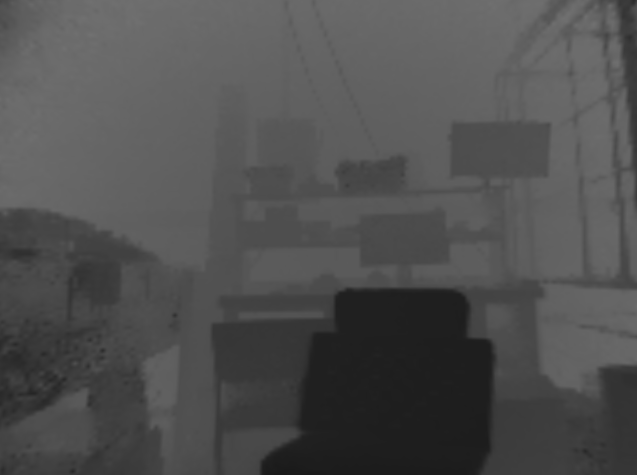
\includegraphics[width=4.8cm]{img/manip_0_0_1_a.png}
\end{subfigure}%
\begin{subfigure}{5cm}
  \centering
  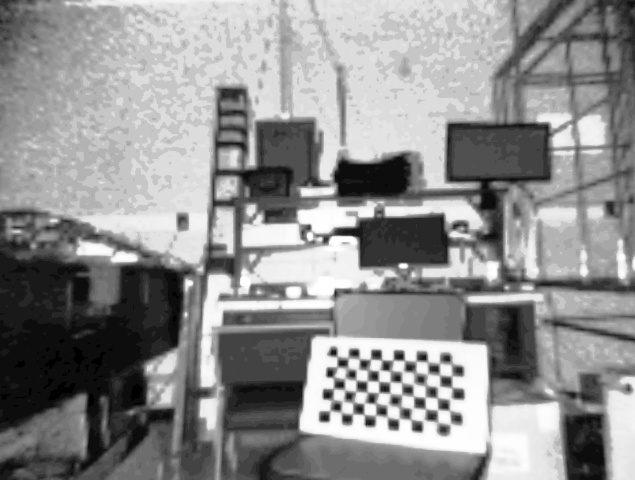
\includegraphics[width=4.8cm]{img/manip_0_0_1_b.png}
\end{subfigure}
\begin{subfigure}{5cm}
  \centering
  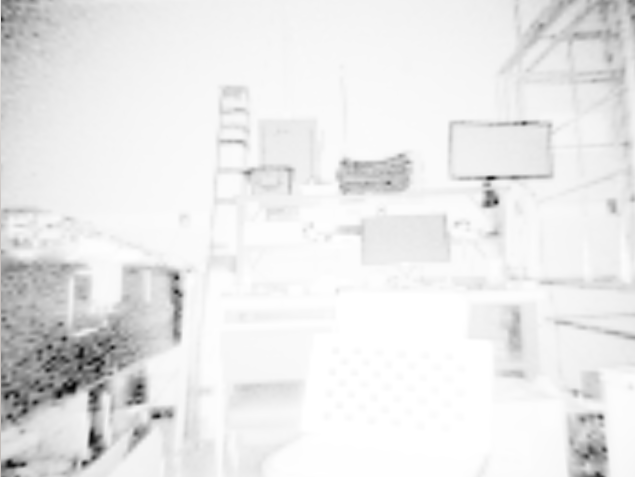
\includegraphics[width=4.8cm]{img/manip_0_0_1_c.png}
\end{subfigure}
\caption{Left: depth image - the darker, the nearer. Center: visual image. Right: confidence image - the variance is high on objects rims (scattering), on the picture edges (sensor limitations) and on some surfaces (thermal noise)}
\label{fig:manip_0_0_1}
\end{center}
\end{figure}
The limited range is highlighted in figure \ref{fig:manip_0_0_2} where an object is put a few centimeters away from the camera. The confidence becomes extremely bad (black) as the measured distance is clearly far from reality.
% figure manip_0_0_2
\begin{figure}[!htt]
\begin{center}
\begin{subfigure}{5cm}
  \centering
  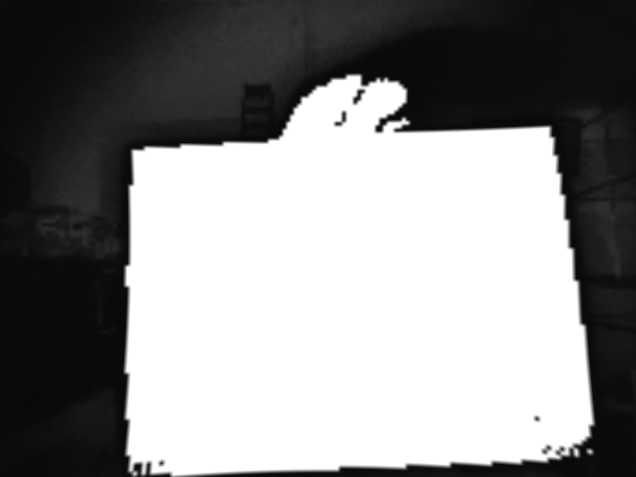
\includegraphics[width=4.8cm]{img/manip_0_0_2_a.png}
\end{subfigure}%
\begin{subfigure}{5cm}
  \centering
  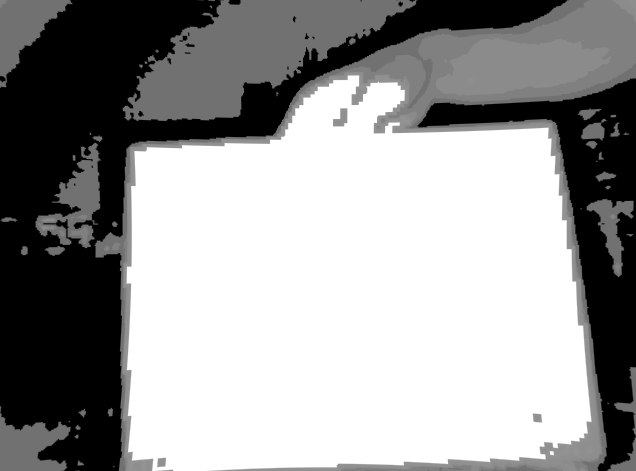
\includegraphics[width=4.8cm]{img/manip_0_0_2_b.png}
\end{subfigure}
\begin{subfigure}{5cm}
  \centering
  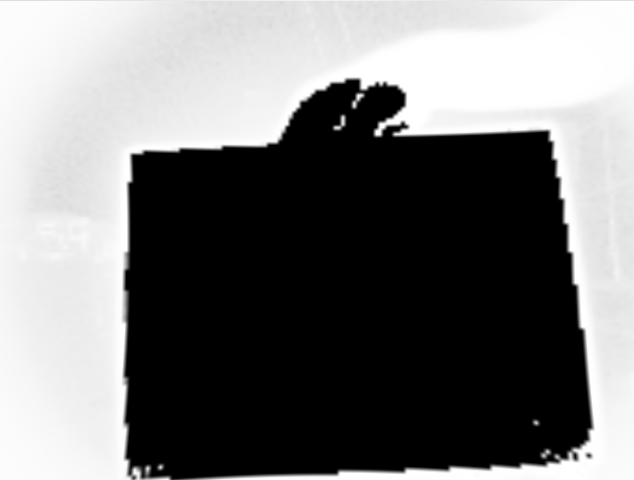
\includegraphics[width=4.8cm]{img/manip_0_0_2_c.png}
\end{subfigure}
\caption{When the object exceed the range limitation of the camera, the measurement can be twisted}
\label{fig:manip_0_0_2}
\end{center}
\end{figure}
In figure \ref{fig:manip_0_0_3}, the same object is held a little farther so it can be measured correctly. However, the low luminosity induces the automatic exposure regulation to wait a little longer during the capture in order to make a good measurement, leading to very noisy pictures when the environment is brighter.
% figure manip_0_0_3
\begin{figure}[!htt]
\begin{center}
\begin{subfigure}{5cm}
  \centering
  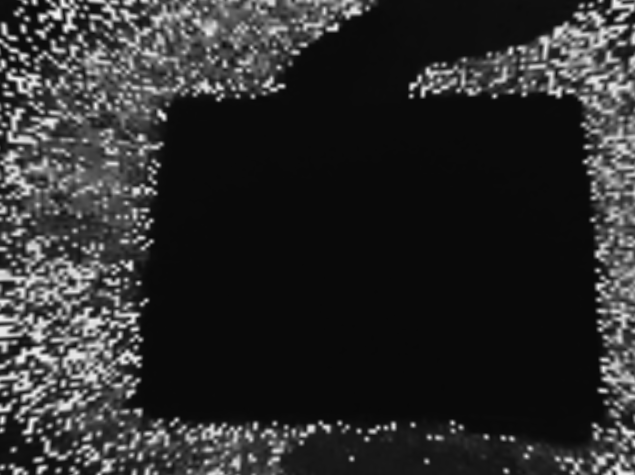
\includegraphics[width=4.8cm]{img/manip_0_0_3_a.png}
\end{subfigure}%
\begin{subfigure}{5cm}
  \centering
  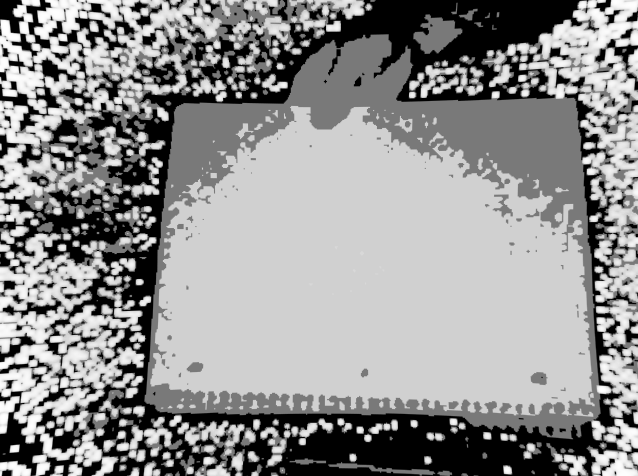
\includegraphics[width=4.8cm]{img/manip_0_0_3_b.png}
\end{subfigure}
\begin{subfigure}{5cm}
  \centering
  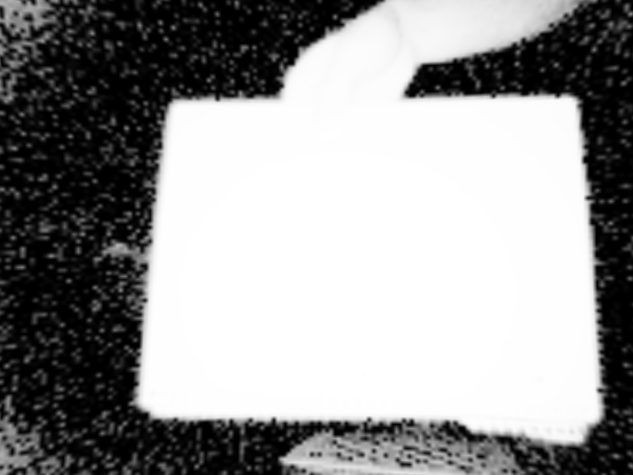
\includegraphics[width=4.8cm]{img/manip_0_0_3_c.png}
\end{subfigure}
\caption{If the object is too close (even if respecting the range limitation), auto-exposure can lead to very high noise in the background}
\label{fig:manip_0_0_3}
\end{center}
\end{figure}
Figure \ref{fig:manip_0_0_4} illustrates that the quality of the measurement is material-dependent. Here, the reflect of an aluminum slab corrupt the depth and visual pictures when the computation of confidence doesn't highlight the problem everywhere on the slab which means that the quality of a measurement cannot be qualified by the confidence picture only.
% figure manip_0_0_4
\begin{figure}[!htt]
\begin{center}
\begin{subfigure}{5cm}
  \centering
  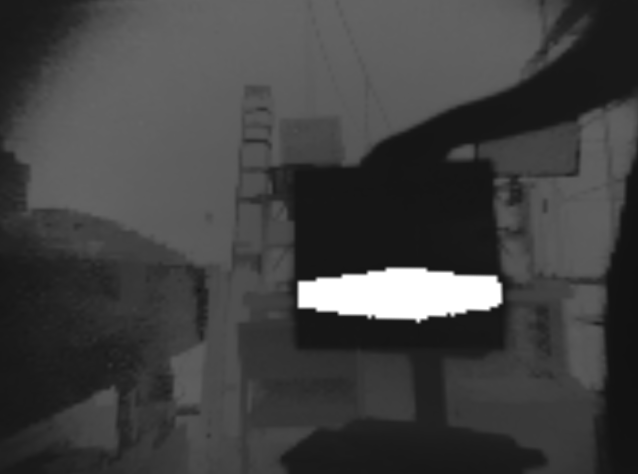
\includegraphics[width=4.8cm]{img/manip_0_0_4_a.png}
\end{subfigure}%
\begin{subfigure}{5cm}
  \centering
  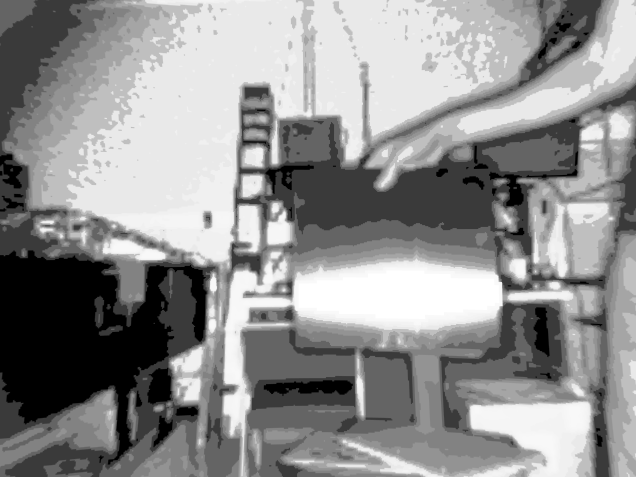
\includegraphics[width=4.8cm]{img/manip_0_0_4_b.png}
\end{subfigure}
\begin{subfigure}{5cm}
  \centering
  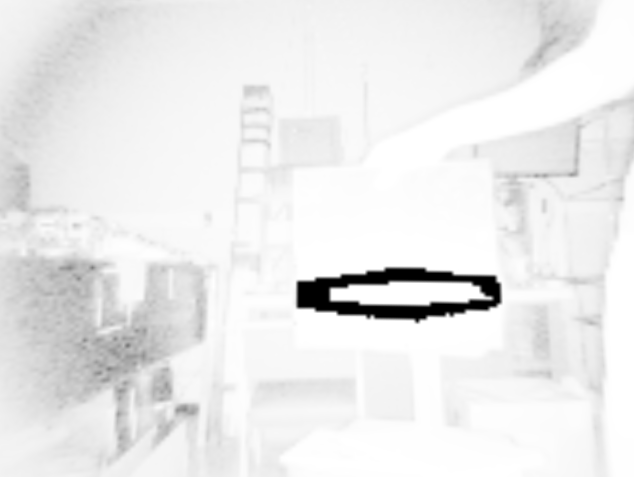
\includegraphics[width=4.8cm]{img/manip_0_0_4_c.png}
\end{subfigure}
\caption{The nature of the material (here some aluminum) changes the reflection properties, hence the measurement quality}
\label{fig:manip_0_0_4}
\end{center}
\end{figure}
Last but not least, the problem of relative movement between the camera and the environment is presented in figure \ref{fig:manip_0_0_5}. On those pictures, a checkerboard is moved with a speed barely higher than a few centimeters per second and leads to very bad results. This can be a very important issue in space where the studied system is supposed to track and analyze the properties of spinning and tumbling targets.
% figure manip_0_0_5
\begin{figure}[!htt]
\begin{center}
\begin{subfigure}{5cm}
  \centering
  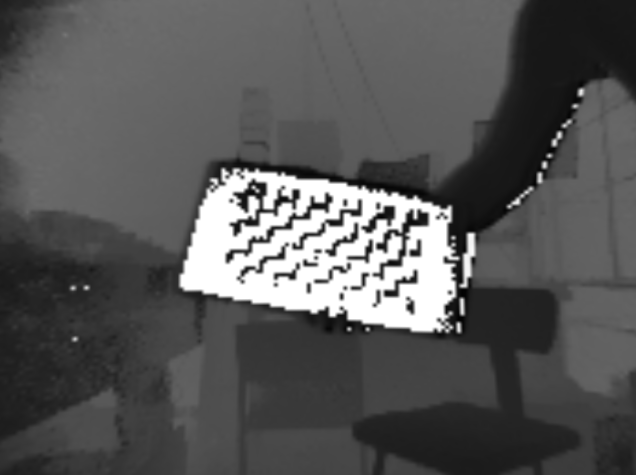
\includegraphics[width=4.8cm]{img/manip_0_0_5_a.png}
\end{subfigure}%
\begin{subfigure}{5cm}
  \centering
  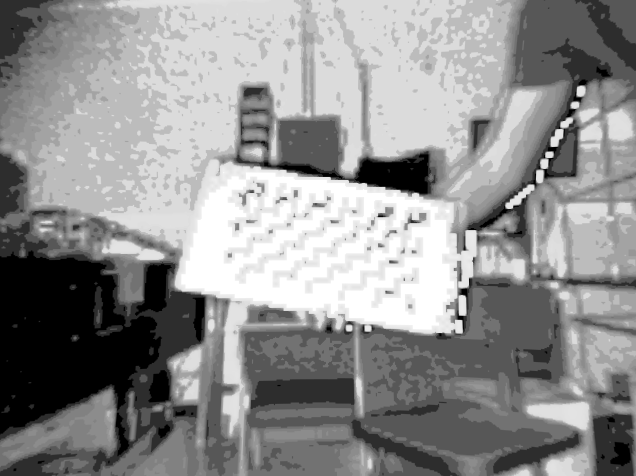
\includegraphics[width=4.8cm]{img/manip_0_0_5_b.png}
\end{subfigure}
\begin{subfigure}{5cm}
  \centering
  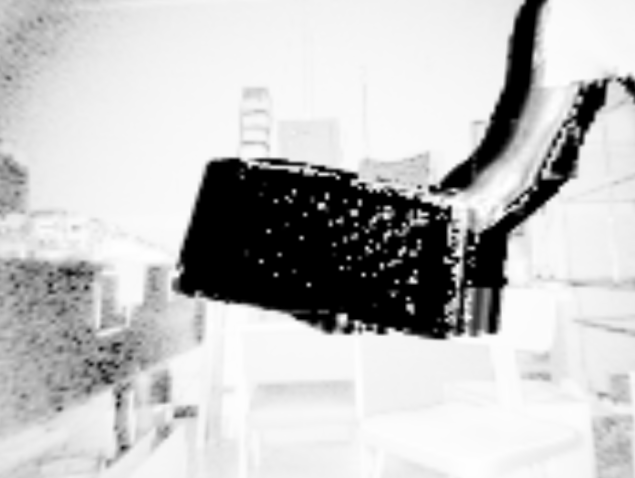
\includegraphics[width=4.8cm]{img/manip_0_0_5_c.png}
\end{subfigure}
\caption{The movement is a decisive factor driving the measurement accuracy. A relative speed of a few dozens of centimeters per second causes a substantial error in the checkerboard depth measurement}
\label{fig:manip_0_0_5}
\end{center}
\end{figure}

\subsection{Calibration and distortions Rectification}
In figure \ref{fig:manip_0_1_1}, many typical pictures are taken in the limits of the space where checkerboards can be detected using only the visual image. From the coordinates of the points, the software gives the following \textit{intrinsic matrix}:
\begin{equation}
\begin{pmatrix}[0.8]
532.74 & 0 & 308.64\\
0 & 490.43 & 222.22\\
0 & 0 & 1
\end{pmatrix}
\end{equation}
Where the distances are in pixels. Given a pixel size of  $40 \mu m$ (see chapter \ref{chapter:intro}) and the picture scaling ratio of 3.68 along $U$ and 3.33 along $V$, we deduce $f_U = 5.9 mm$ and $f_V = 5.9 mm$ where the small differences with the values as provided by the constructor can be explained by a variable focal length. Beside, $c_U = 308$ and $c_V = 222$ are not far from the theoretical center $c_U = 320$ and $c_V = 240$. The distortion coefficients are equals to:
\begin{equation}
\label{eq:intrinsic}
\begin{pmatrix}[0.8]
-3.45e-01 & 1.44e-01 &-2.20e-04 & 1.91e-03 & 5.181e-02
\end{pmatrix}
\end{equation}
Figure \ref{fig:manip_0_1_2} shows the result after the distortion rectification for a very close object.

% Figure manip_0_1_1
\begin{figure}[!htt]
\begin{center}
\begin{subfigure}{5cm}
  \centering
  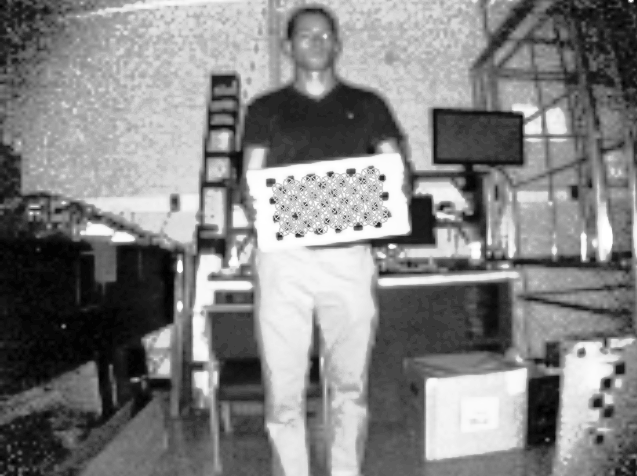
\includegraphics[width=4.8cm]{img/manip_0_1_1_a.png}
\end{subfigure}%
\begin{subfigure}{5cm}
  \centering
  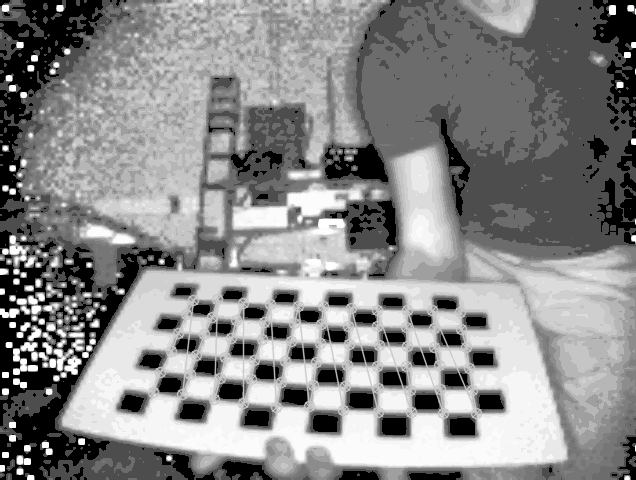
\includegraphics[width=4.8cm]{img/manip_0_1_1_b.png}
\end{subfigure}
\begin{subfigure}{5cm}
  \centering
  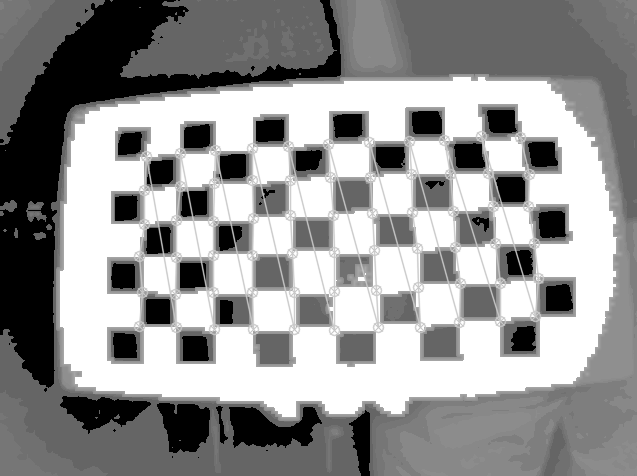
\includegraphics[width=4.8cm]{img/manip_0_1_1_c.png}
\end{subfigure}
\caption{We vary the checkerboard orientation to the limits of the detection to cover the space at maximum. Left: the farthest distance. Center: the maximal inclination. Right: the closest distance}
\label{fig:manip_0_1_1}
\end{center}
\end{figure}
% Figure manip_0_1_2
\begin{figure}[!htt]
\begin{center}
\begin{subfigure}{5cm}
  \centering
  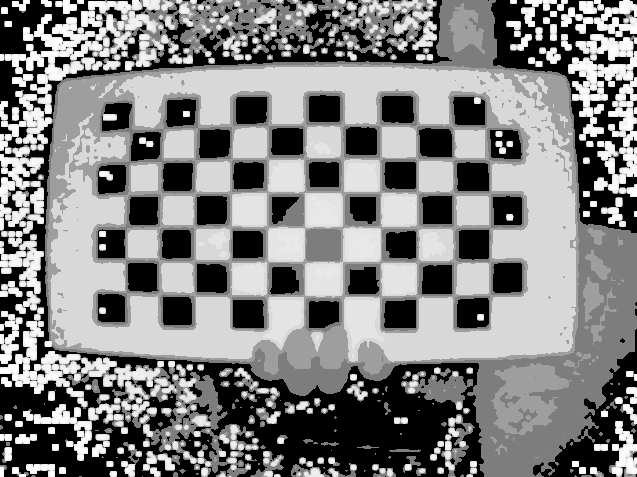
\includegraphics[width=4.8cm]{img/manip_0_1_2_a.png}
\end{subfigure}%
\begin{subfigure}{5cm}
  \centering
  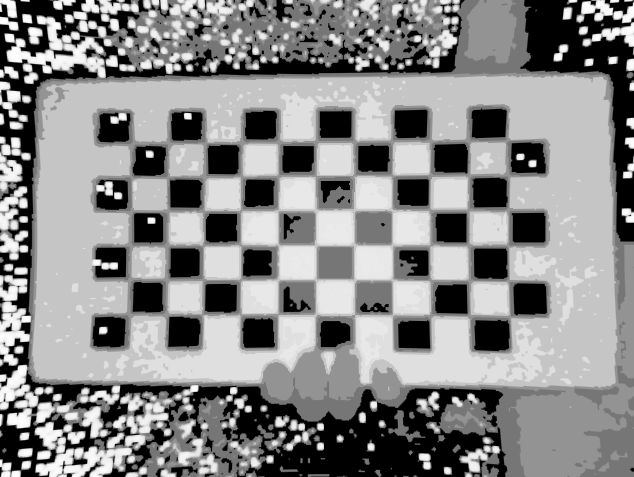
\includegraphics[width=4.8cm]{img/manip_0_1_2_b.png}
\end{subfigure}
\caption{Left: a checkerboard before rectification. Right: the same checkerboard after the distortions rectification. The edges are now straight and parallel}
\label{fig:manip_0_1_2}
\end{center}
\end{figure}
\subsection{Absolute Depth Measurement}
In this paragraph, one of the example implemented with this project software is used to compute the depth of a calibration target situated $1m$ away from the \gls{ORF} camera (figure \ref{fig:manip_0_2_1}). 
% Figure fig:manip_0_2_1
\begin{figure}[!htt]
\begin{center}
  \centering
  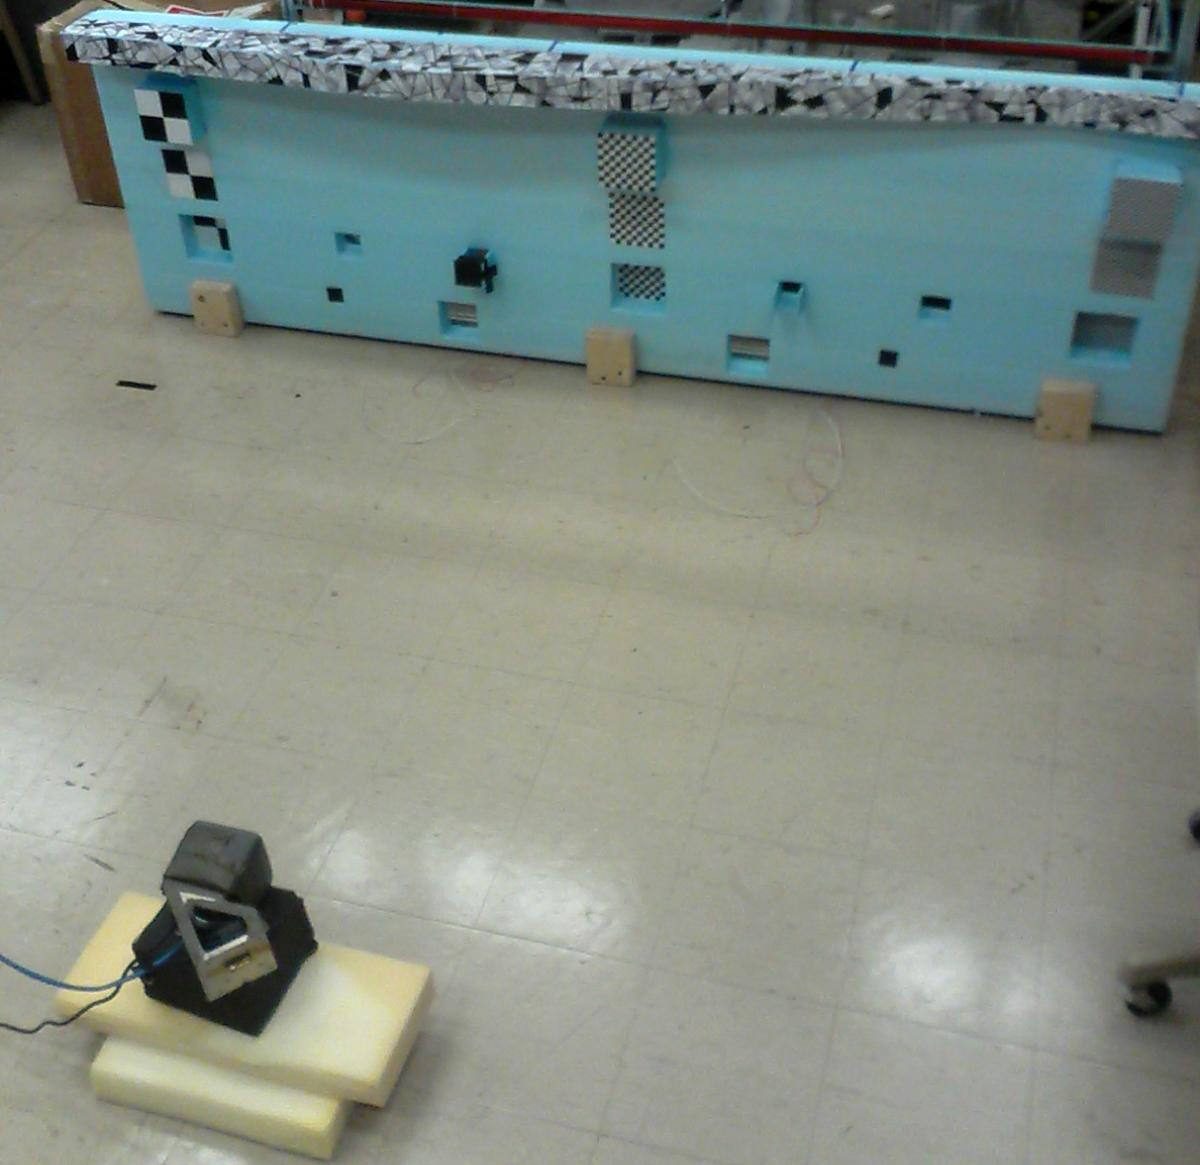
\includegraphics[width=7cm]{img/orf_meas_setup.jpg}
\caption{The setup used for \gls{ORF} calibration}
\label{fig:manip_0_2_1}
\end{center}
\end{figure}
To take the noise into account, the capture of figure \ref{fig:manip_0_2_2} is realized several times to compensate the thermal noise of $1.026mm$. This difference of a few millimeters is explained by the inaccuracy of the setup itself, the material reflectivity, and the fact that the measured point is not directly in the focal axis (we then measure the hypothesis as presented in figure \ref{fig:orf_depth})
% Figure fig:manip_0_2_2
\begin{figure}[!htt]
\begin{center}
\begin{subfigure}{5cm}
  \centering
  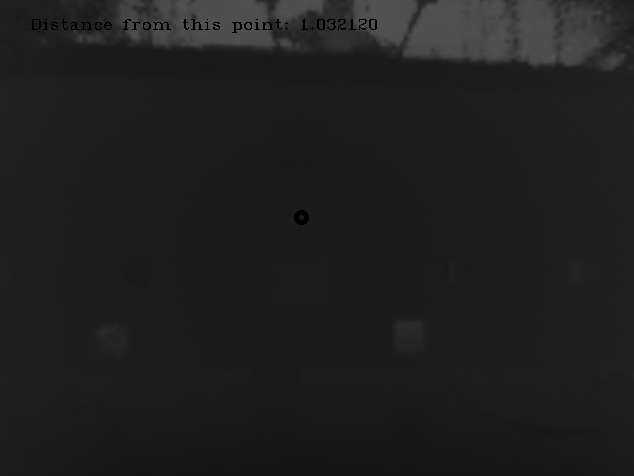
\includegraphics[width=4.8cm]{img/manip_0_2_2_a.png}
\end{subfigure}%
\begin{subfigure}{5cm}
  \centering
  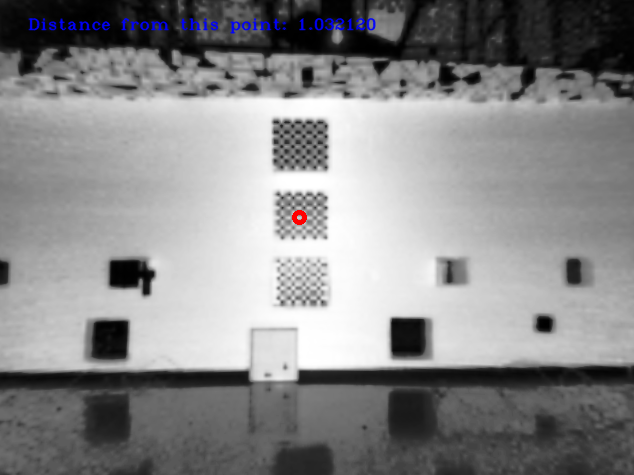
\includegraphics[width=4.8cm]{img/manip_0_2_2_b.png}
\end{subfigure}
\begin{subfigure}{5cm}
  \centering
  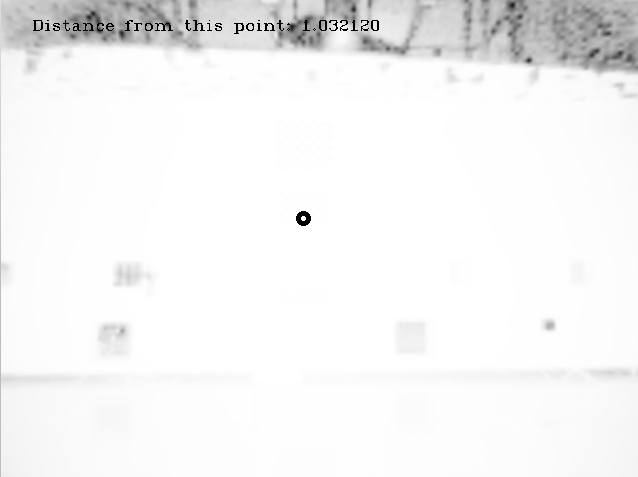
\includegraphics[width=4.8cm]{img/manip_0_2_2_c.png}
\end{subfigure}
\caption{Several measurement are effectuated in the center of the target and their mean is computed to compensate Gaussian noise}
\label{fig:manip_0_2_2}
\end{center}
\end{figure}
This last effect is showed in figure \ref{fig:manip_0_2_3}, where the measured depth is equal to $1.159m$ when the $Z$ coordinate should be still about $1m$.
% Figure fig:manip_0_2_3
\begin{figure}[!htt]
\begin{center}
\begin{subfigure}{5cm}
  \centering
  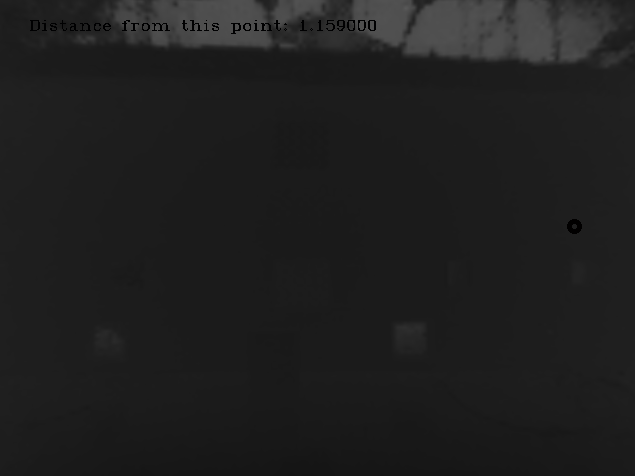
\includegraphics[width=4.8cm]{img/manip_0_2_3_a.png}
\end{subfigure}%
\begin{subfigure}{5cm}
  \centering
  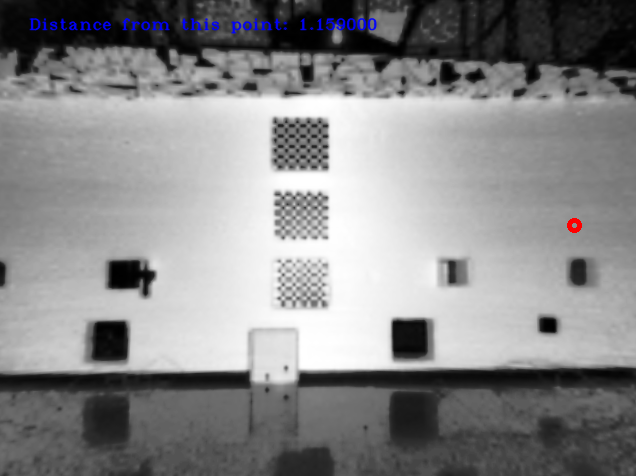
\includegraphics[width=4.8cm]{img/manip_0_2_3_b.png}
\end{subfigure}
\begin{subfigure}{5cm}
  \centering
  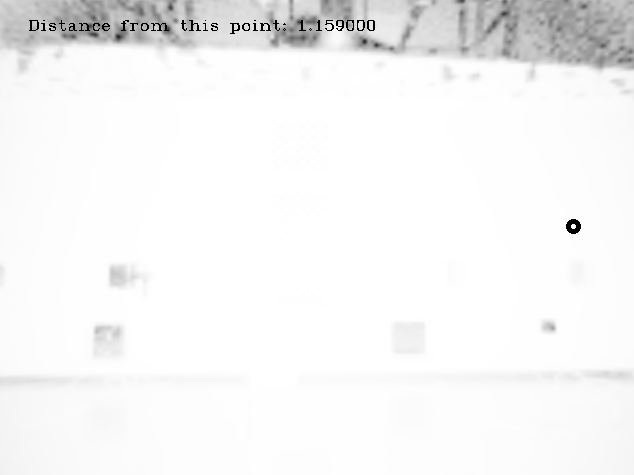
\includegraphics[width=4.8cm]{img/manip_0_2_3_c.png}
\end{subfigure}
\caption{The same measurement are made on the right of the target to illustrate the problem of $XYZ$ reconstruction from the depth}
\label{fig:manip_0_2_3}
\end{center}
\end{figure}

\subsection{Relative Depth Measurement}
Using the data of the two last paragraphs, we can also compute $XYZ$ coordinates in the $T$ coordinate system using pinhole inversion. This time, we perform 6 captures in three targets presenting a relative difference of $2 inches$ in $Z$ coordinates and we compute this relative distance to get rid of the systemic error in the setup accuracy (figure \ref{fig:manip_0_3_1}). We obtain then:
%Figure manip_0_3_1
\begin{figure}[!htt]
\begin{center}
\begin{subfigure}{5cm}
  \centering
  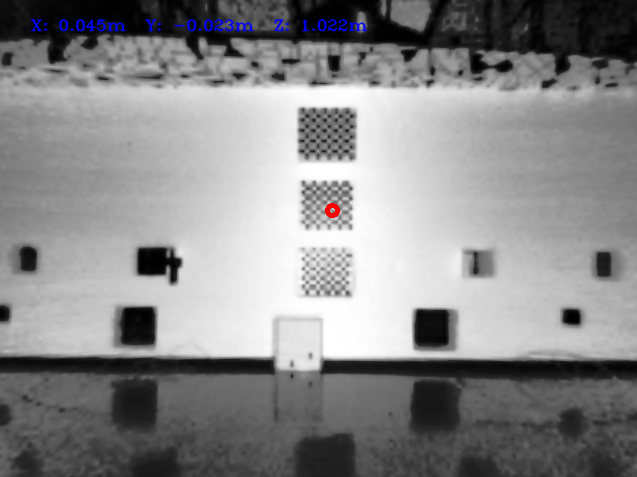
\includegraphics[width=4.8cm]{img/manip_0_3_1_a.png}
\end{subfigure}%
\begin{subfigure}{5cm}
  \centering
  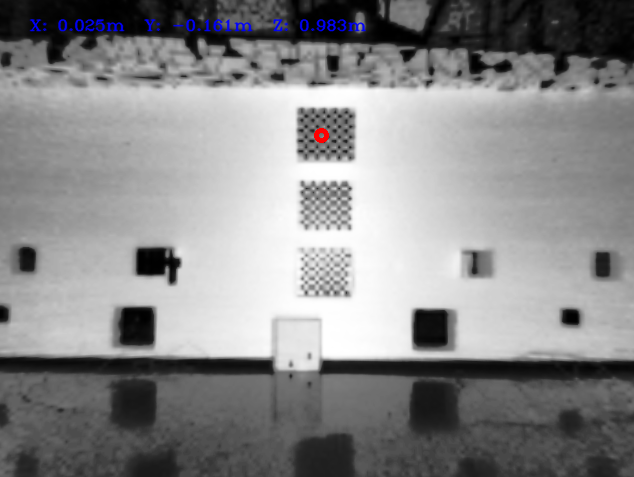
\includegraphics[width=4.8cm]{img/manip_0_3_1_b.png}
\end{subfigure}
\begin{subfigure}{5cm}
  \centering
  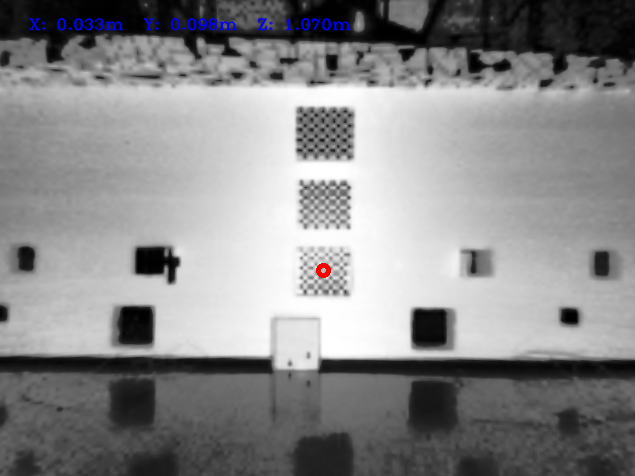
\includegraphics[width=4.8cm]{img/manip_0_3_1_c.png}
\end{subfigure}
\caption{The mean $XYZ$ coordinates are computed for three different points to deduce the relative $Z$ distance between them and compare it to the reference benchmark}
\label{fig:manip_0_3_1}
\end{center}
\end{figure}
To be more generalist and verify that $X$ and $Y$ coordinates are also correct (unlike $Z$, they depends on $f_U$, $f_V$, $c_U$, $c_V$) we can also measure the euclidean distance between two vertexes of a target with a known geometry framed by a camera with a random angle and distance (figure \ref{fig:manip_0_3_2}). Once again, this experiment is repeated several times and the mean distance is computed:
\begin{equation}
\bar{d} = \sqrt{(\bar{x_1} - \bar{x_2})^2 + (\bar{y_1} - \bar{y_2})^2 + (\bar{z_1} - \bar{z_2})^2} = 6.24 cm
\end{equation}
Which is blaaaaaa compared to the blaaaaa we was supposed to obtain.
%Figure manip_0_3_2
\begin{figure}[!htt]
\begin{center}
\begin{subfigure}{5cm}
  \centering
  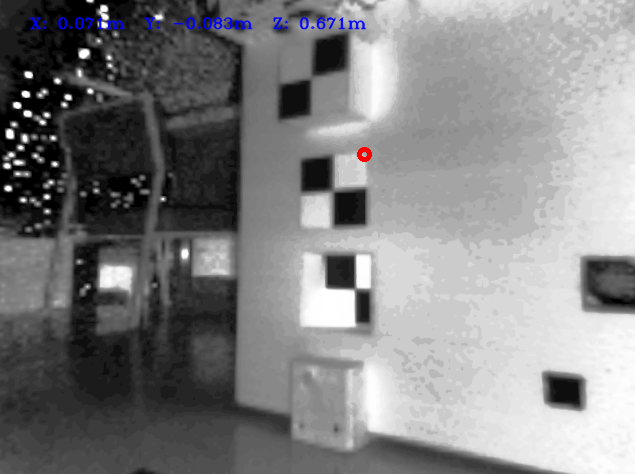
\includegraphics[width=4.8cm]{img/manip_0_3_2_a.png}
\end{subfigure}%
\begin{subfigure}{5cm}
  \centering
  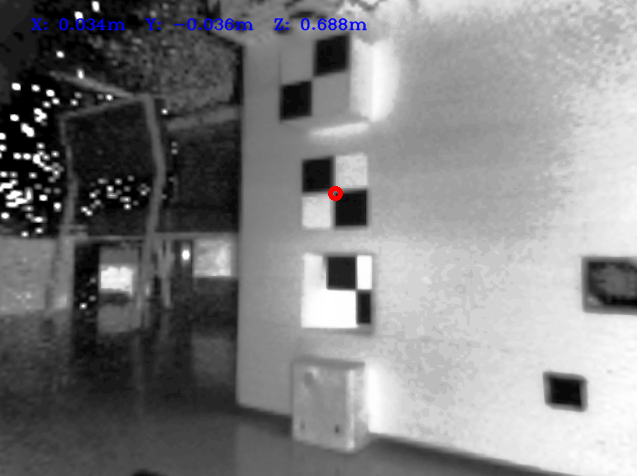
\includegraphics[width=4.8cm]{img/manip_0_3_2_b.png}
\end{subfigure}
\caption{The mean $XYZ$ coordinates are computed for two different points to deduce the euclidean distance between them and compare it to the reference benchmark}
\label{fig:manip_0_3_2}
\end{center}
\end{figure}


\subsection{3D Points Cloud Construction}
In these last experiments, a point cloud is constructed using the \gls{PCL} library tools included in the software developed in this project. In figure \ref{fig:manip_0_4_1}, two view of the same points cloud are given. We can notice that the visual image is included in the process since we can see the pattern on the checkerboard. The importance of the scattering and the thermal noise can be highlighted especially if we look precisely to the edges of the checkerboard and its shape from above (which is supposed to be flat).
%Figure manip_0_4_1
\begin{figure}[!htt]
\begin{center}
\begin{subfigure}{7cm}
  \centering
  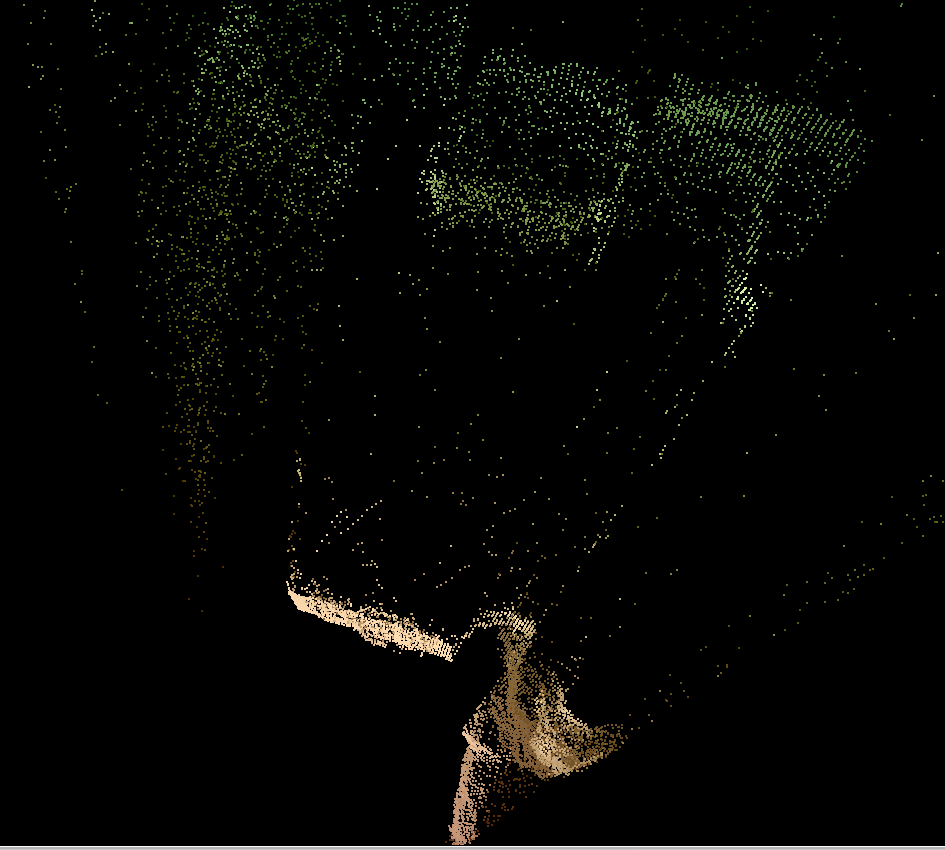
\includegraphics[width=6.8cm]{img/manip_0_4_1_a.png}
\end{subfigure}%
\begin{subfigure}{7cm}
  \centering
  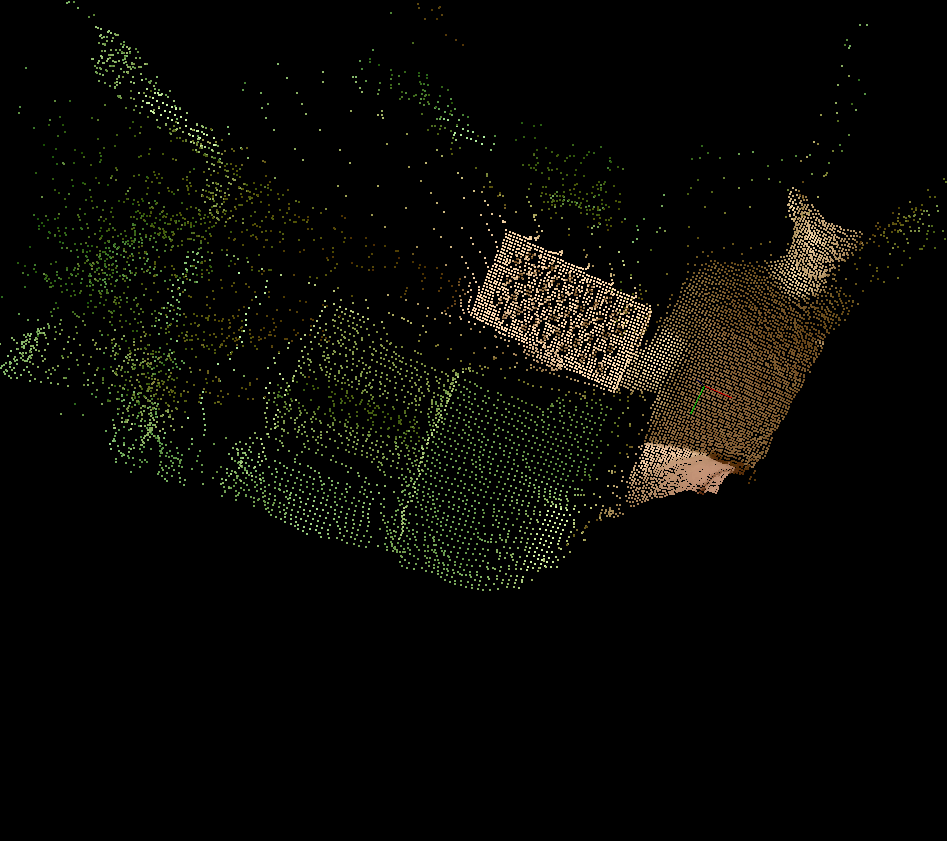
\includegraphics[width=6.8cm]{img/manip_0_4_1_b.png}
\end{subfigure}
\caption{A 3D points cloud with visual information reconstructed from \gls{ORF} pictures. Scattering around edges and thermal noise in the background can be observed}
\label{fig:manip_0_4_1}
\end{center}
\end{figure}
Figure \ref{fig:manip_0_4_2} illustrates the importance of the noise due to auto-exposure when an object is very close to the lens.
%Figure manip_0_4_2
\begin{figure}[!htt]
\begin{center}
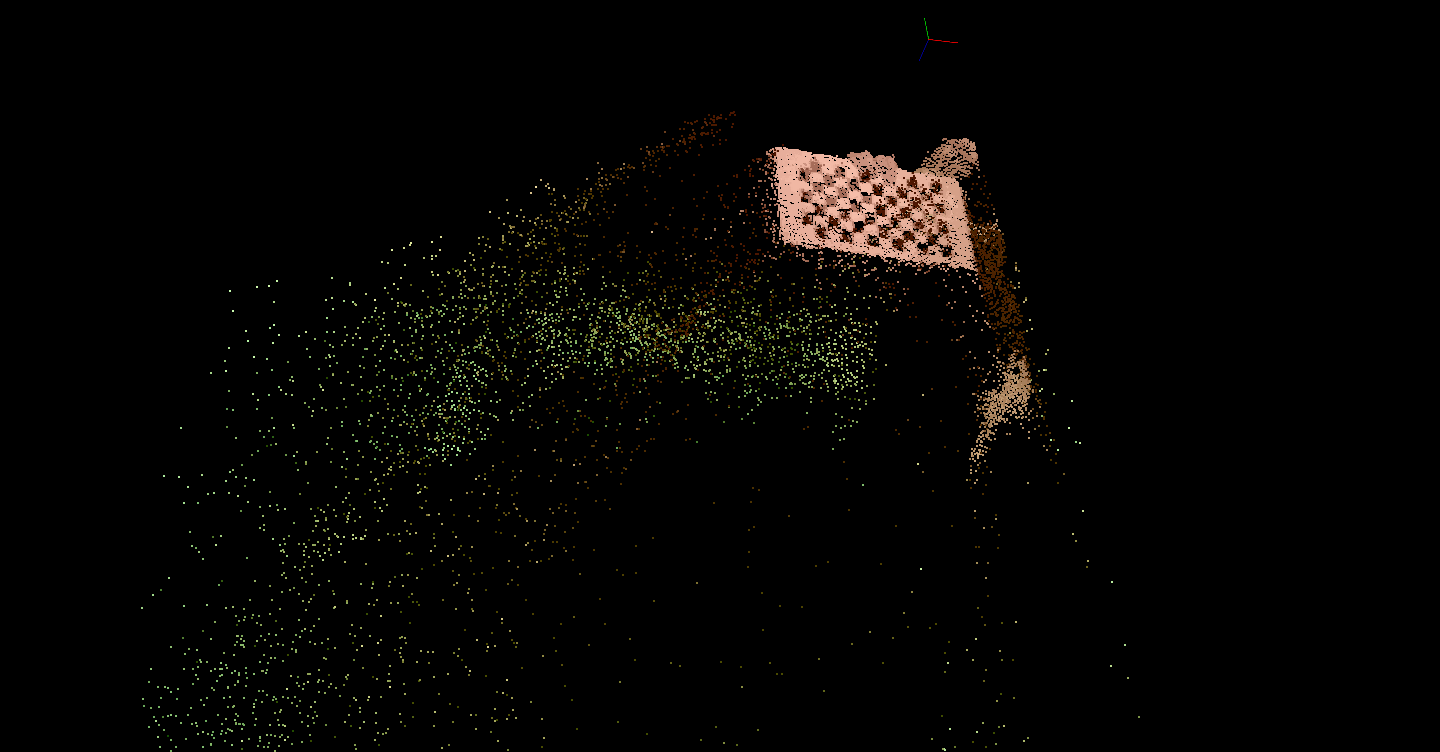
\includegraphics[width=10cm]{img/manip_0_4_2.png}
\caption{When the target is too close from the camera, the background becomes very noisy because of the auto-exposure}
\label{fig:manip_0_4_2}
\end{center}
\end{figure}

\section{Stereo Acquisition}
In this section, we will discuss the efficiency of the VERTIGO sensors and algorithm. As a lot of work has already been done on the subject, for instance in \cite{vertigo_phd}, \cite{muggler_phd} and \cite{makowka_phd}, this project simply focused on the comparison with the \gls{ORF} camera and points out the complementarity of the two systems.

The reconstruction of a 3D points cloud from stereo sensors is performed through the elaboration of a disparity map, whose information is quite similar to the one of the \gls{ORF} depth map. To create this disparity map, different techniques can be used, a taxonomy of those is given in \cite{stereo_methods_comparaison}. Basically, the process always implies the following steps: features detection and matching, aggregation, disparity computation and optimization. The quality of the disparity image is the dependent on the number of matchable features, called supporting points, in the left and right pictures: if the considered environment is highly textured, this will lead to accurate 3D reconstruction while uniform patches won't give reliable results. The interstices between supporting points is filled by aggregation methods around those points which have also a lot of influence on the final disparity map. In figure \ref{manip_1_1}, the results of a block matching stereo function provided in OpenCV libraries illustrate our remarks.

However, if the stereo vision algorithms suffer from this texture dependency, they don't encounter the same defaults as the \gls{ORF} in term of movement and luminosity conditions. This complementarity has been proved qualitatively with the use of a setup involving the \gks{ORF} and the VERTIGO goggles capturing simultaneous pictures of the same object. In figure \ref{manip_1_2}, the movement reliability is highlighted: a checkerboard animated with a speed of the few dozen of centimeters per second is captured by the two sensors. Even if the stereo images could be considered a little more blurred than in the static case, they are still very good and 
la ou l'orf est mauvais, le stereo est bon. C'est le cas du mouvement. Si l'environement bouge rapidement par rappoirt a la camera, pas de problme.

De meme, moins sensible aux conditions lumineuses et aux materiaux utilises.

\section{Multi-sensors Calibration}
To determine the performances of the calibration algorithm we discussed in section \ref{subsec:system_calib}, we connect the \gls{ORF} and the stereo cameras to the VERTIGO computer and we acquire synchronous images of a checkerboard (figure \ref{fig:manip_2_1}. It is important for each capture to make sure the checkerboard is not moving and the luminous conditions are sufficient by checking the confidence picture (figure \ref{fig:manip_2_2}).

% Figure manip_2_1
\begin{figure}[!htt]
\begin{center}
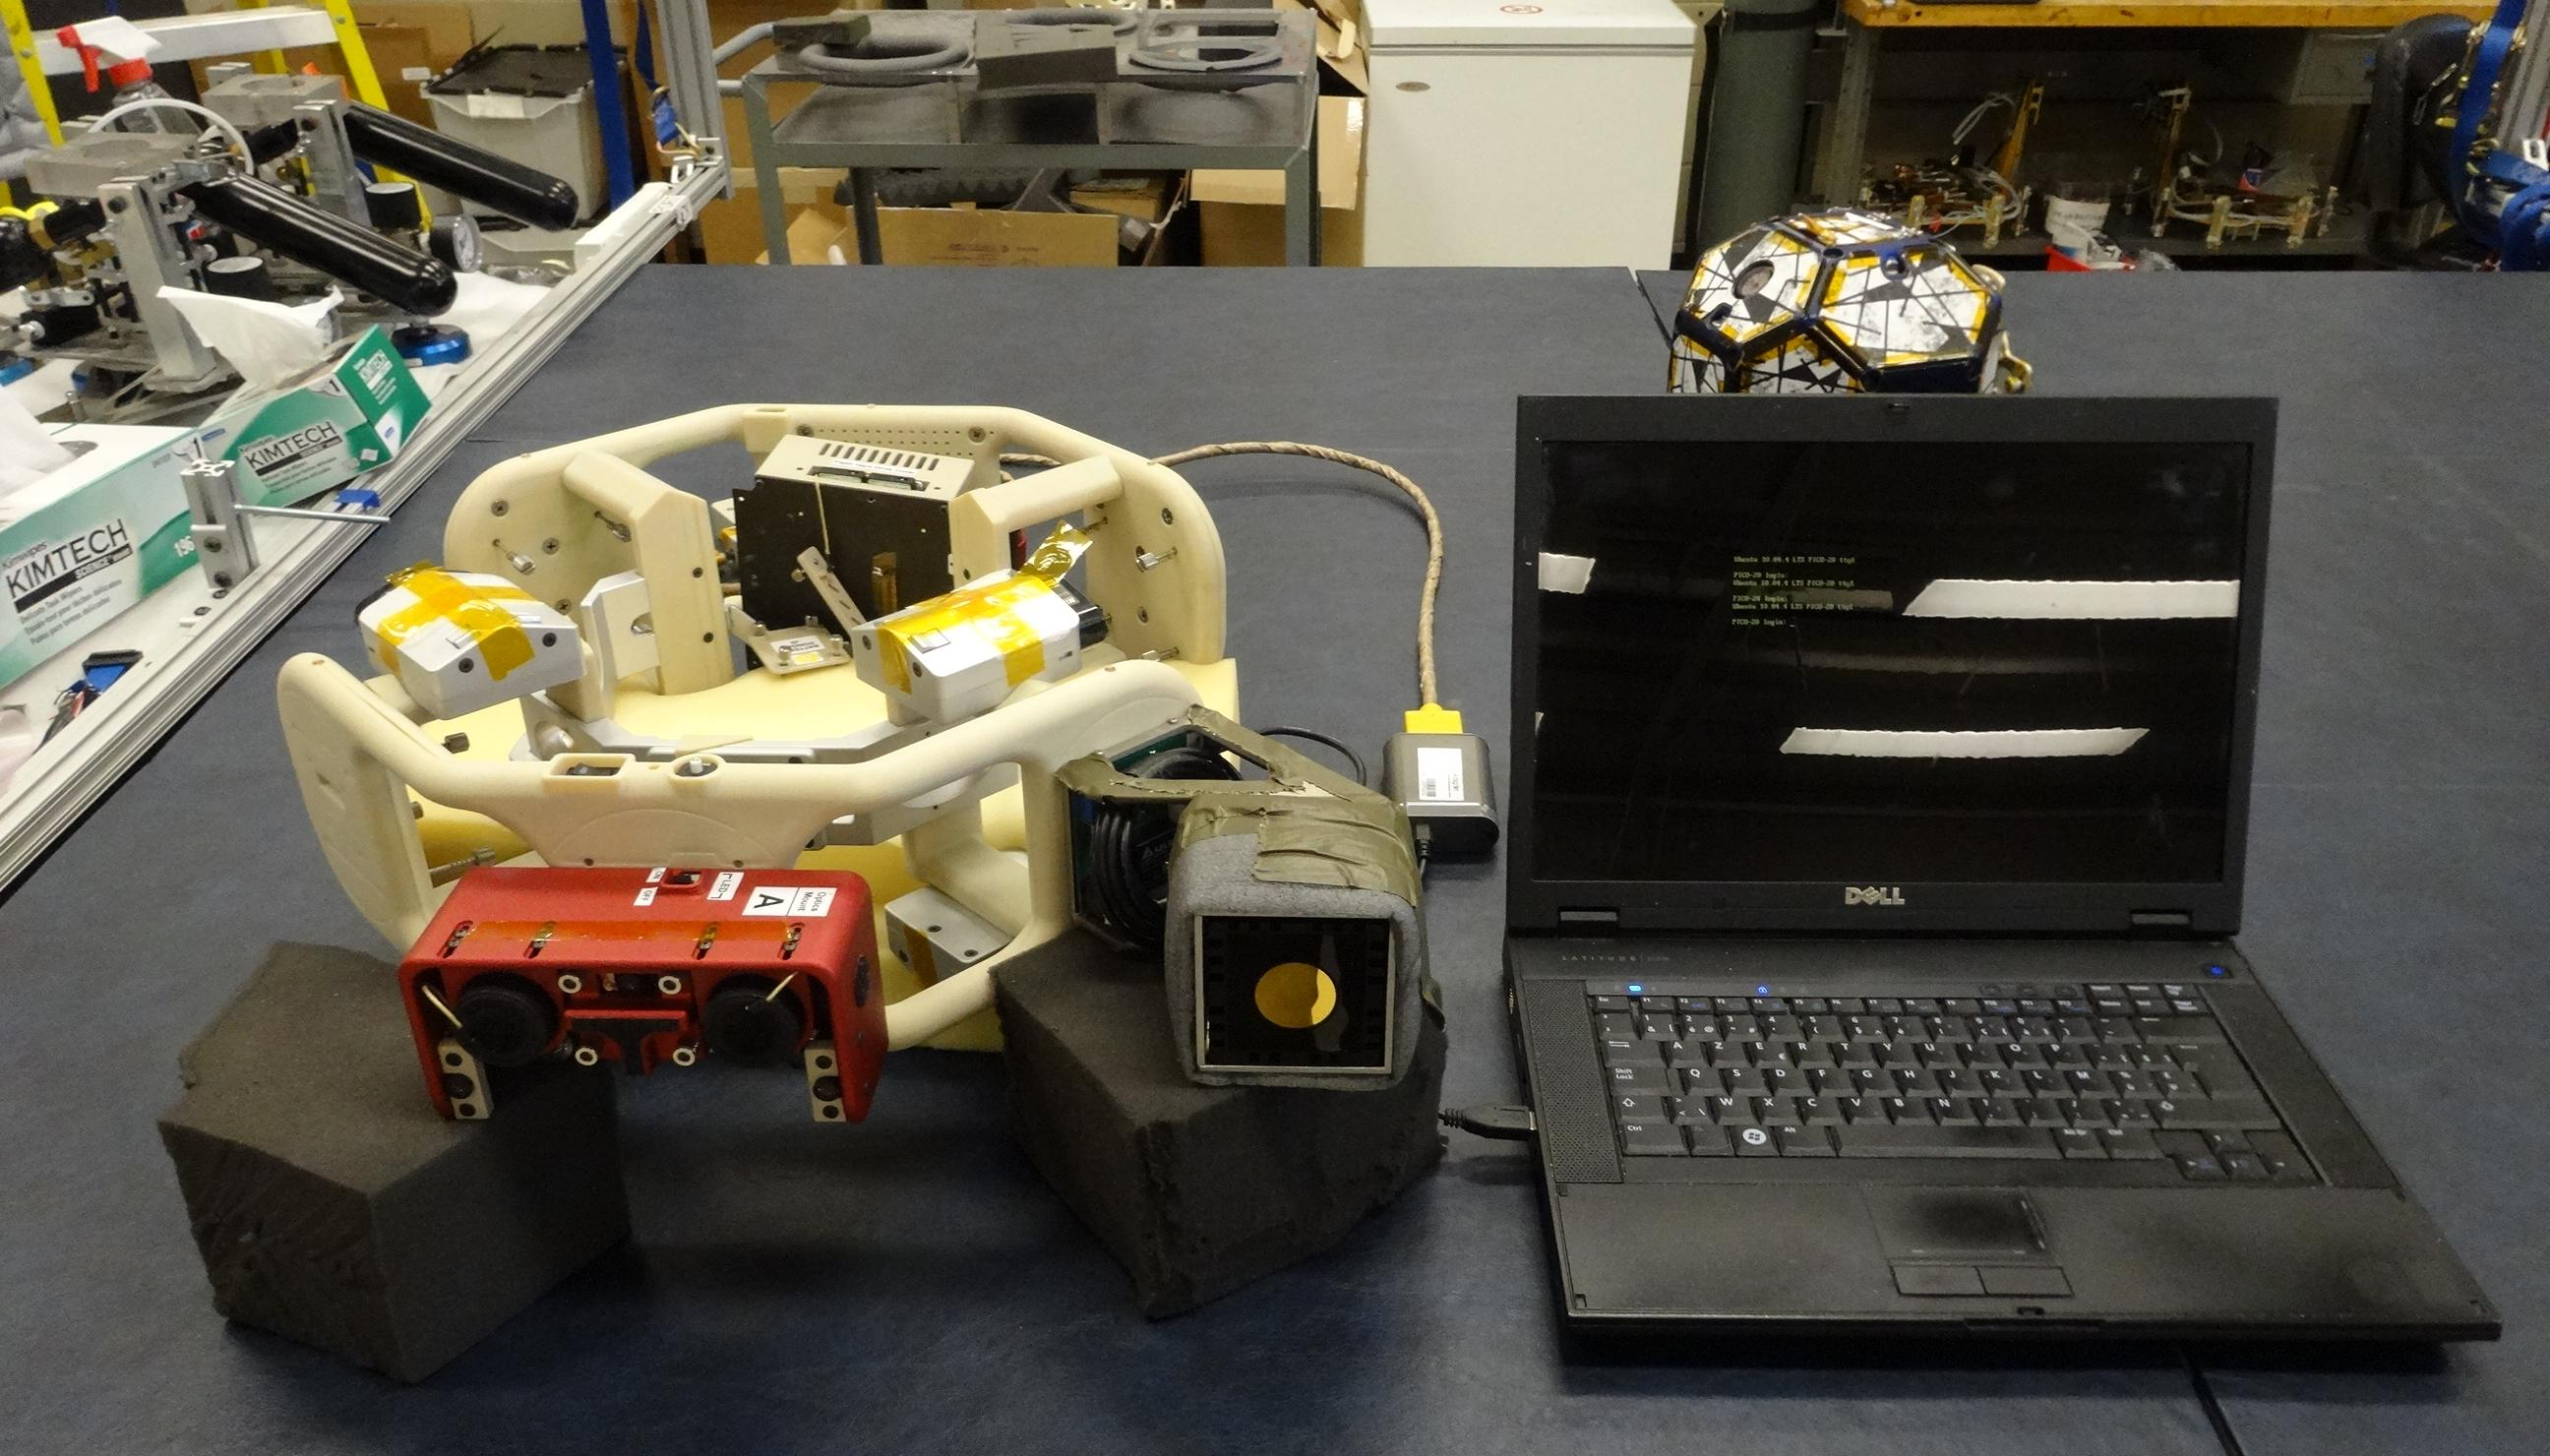
\includegraphics[width=10cm]{img/manip_2_1.jpg}
\caption{The experiment setup: VERTIGO and the ORF camera fixed to the Halo and plugged to the embedded computer}
\label{fig:manip_2_1}
\end{center}
\end{figure}
% Figure manip_2_2
\begin{figure}[!htt]
\begin{center}
\begin{subfigure}{3cm}
  \centering
  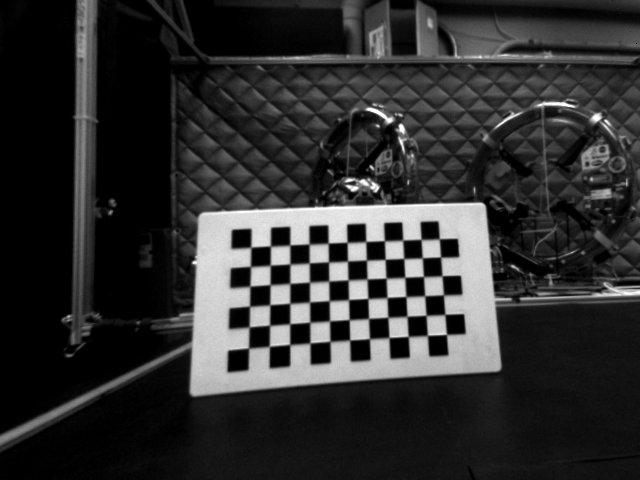
\includegraphics[width=2.8cm]{img/manip_2_2_a.png}
\end{subfigure}%
\begin{subfigure}{2.9cm}
  \centering
  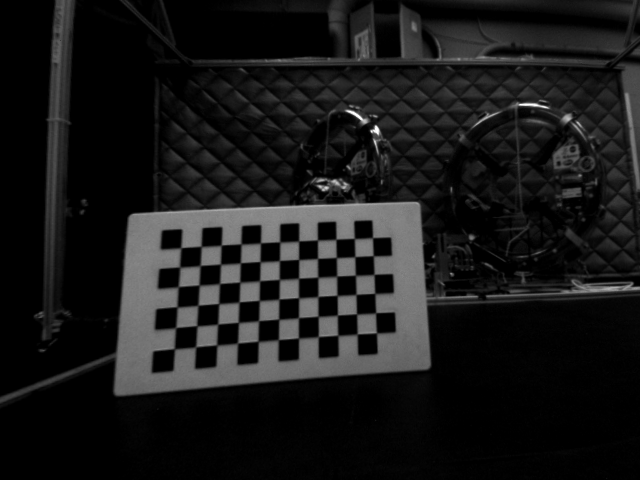
\includegraphics[width=2.8cm]{img/manip_2_2_b.png}
\end{subfigure}
\begin{subfigure}{2.9cm}
  \centering
  
\includegraphics[width=2.8cm]{img/manip_2_2_c.png}
\end{subfigure}
\begin{subfigure}{2.9cm}
  \centering
  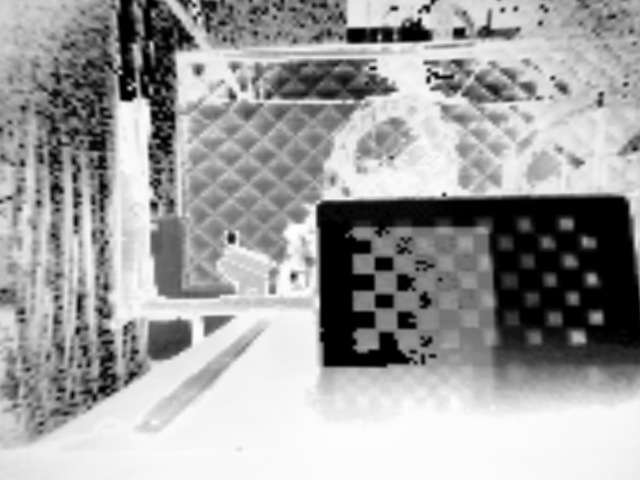
\includegraphics[width=2.8cm]{img/manip_2_2_d.png}
\end{subfigure}
\begin{subfigure}{2.9cm}
  \centering
  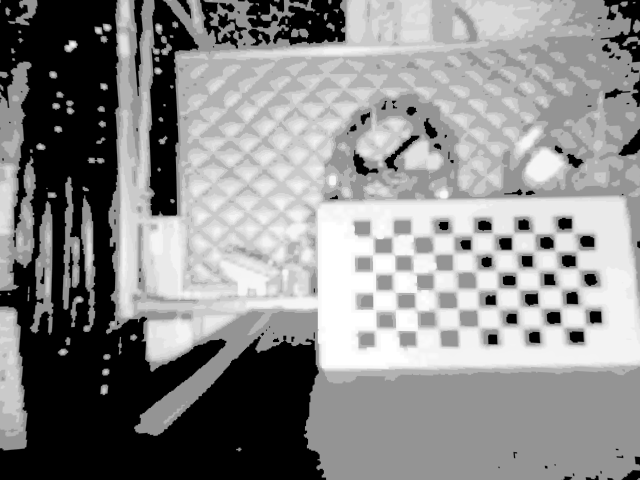
\includegraphics[width=2.8cm]{img/manip_2_2_e.png}
\end{subfigure}
\vspace{0.5cm}
\begin{subfigure}{3cm}
  \centering
  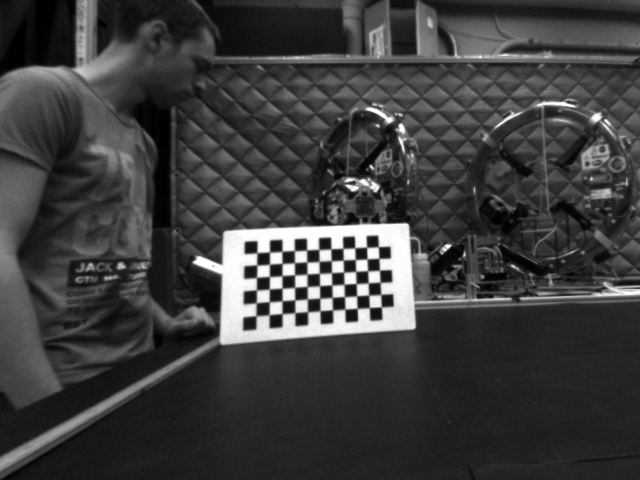
\includegraphics[width=2.8cm]{img/manip_2_2_f.png}
\end{subfigure}%
\begin{subfigure}{2.9cm}
  \centering
  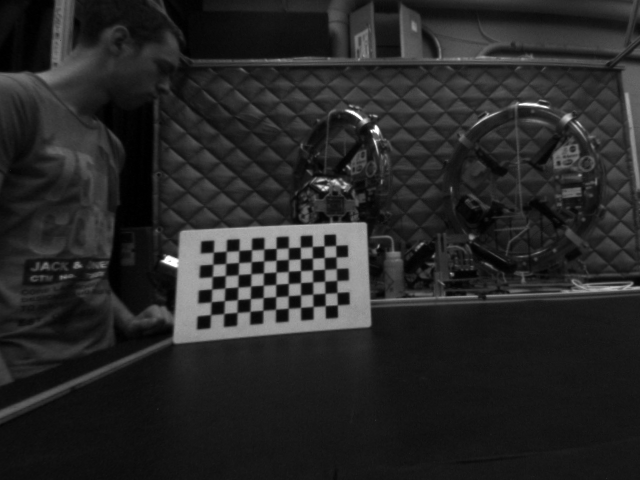
\includegraphics[width=2.8cm]{img/manip_2_2_g.png}
\end{subfigure}
\begin{subfigure}{2.9cm}
  \centering
  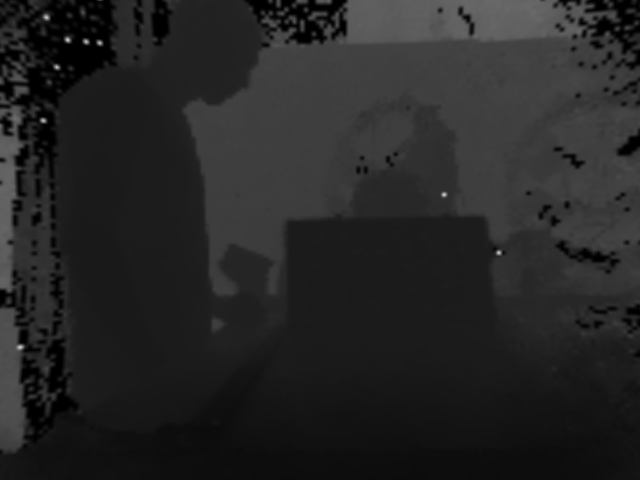
\includegraphics[width=2.8cm]{img/manip_2_2_h.png}
\end{subfigure}
\begin{subfigure}{2.9cm}
  \centering
  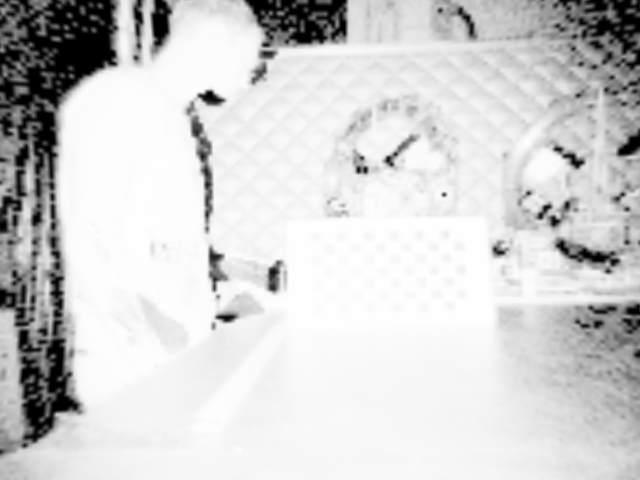
\includegraphics[width=2.8cm]{img/manip_2_2_i.png}
\end{subfigure}
\begin{subfigure}{2.9cm}
  \centering
  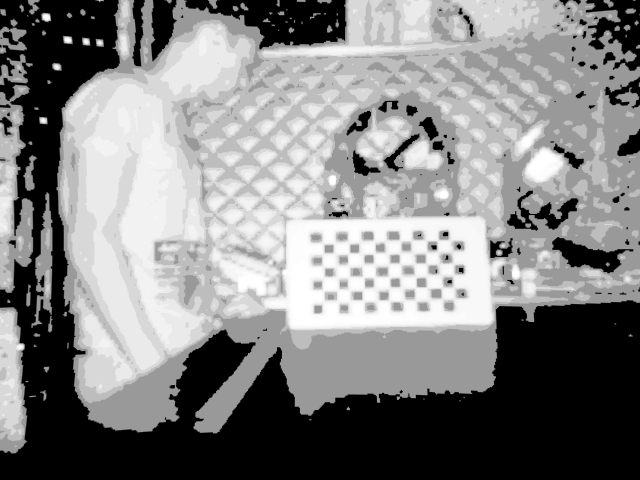
\includegraphics[width=2.8cm]{img/manip_2_2_j.png}
\end{subfigure}
\caption{Above: a bad capture for calibration (from left to right: left image, right image, depth image, confidence image, ORF visual image). Below: a good capture (same meaning)}
\label{fig:manip_2_2}
\end{center}
\end{figure}
We then proceed to corner detection in those images and reconstruct separately the 3D corresponding points for the \gls{ORF} (in the $T$ coordinate system) and the stereo cameras (in the $L$ coordinate system). The transformation matrix between them being still unknown, those points are represented in the same 3D visualization assuming a common origin (figure \ref{fig:manip_2_3}). 
% Figure manip_2_3
\begin{figure}[!htt]
\begin{center}
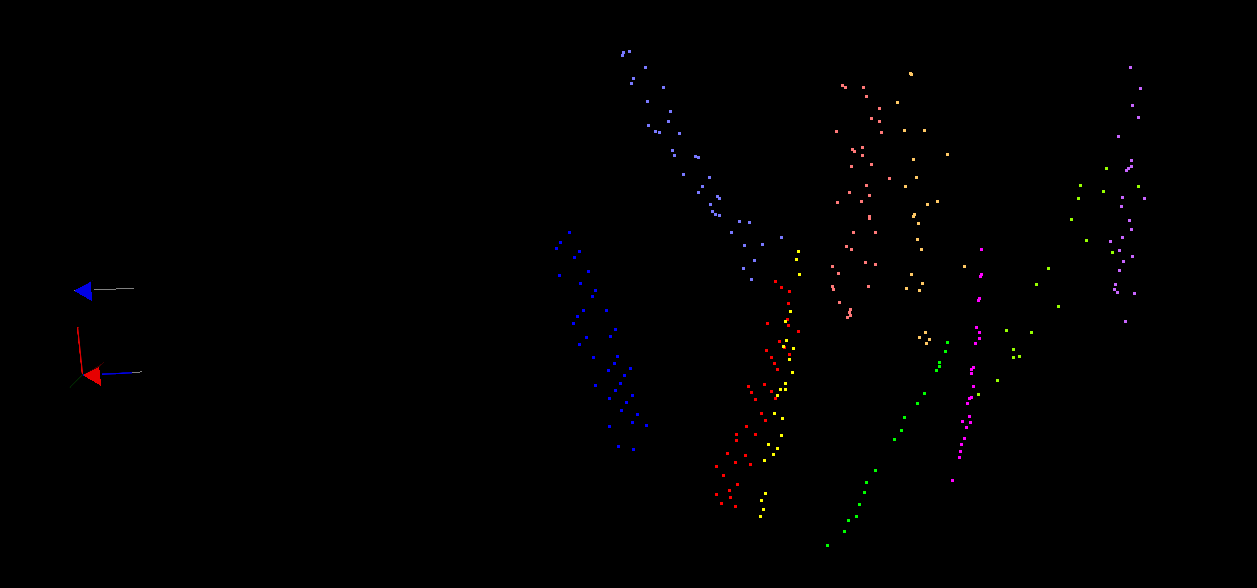
\includegraphics[width=14cm]{img/manip_2_3.png}
\caption{ORF and stereo reconstructed checkerboard are represented on the same image. Dark blue: stereo board 1. Light blue: ORF board 1. Red: stereo board 2. Rose: ORF board 2. Yellow: stereo board 3. Orange: ORF board 3. Dark green: stereo board 4. Light green: ORF board 4. Dark violet: stereo board 5. Light violet: ORF board 5}
\label{fig:manip_2_3}
\end{center}
\end{figure}
It is important to understand though that this has no physical meaning, it is just a way to verify a few parameters like the size of the cloud, the regularity of the checkerboard, their straightness, the noise,... For example, we can notice, the noise more important with the \gls{ORF} as predicted theoretically (figure \ref{fig:manip_2_4}). Hopefully, the RANSAC scheme will help to put aside the points that are too distant each other. Concerning the point evaluated by the stereo sensors, they are more accurate since the triangulation process is based on the feature matching which is supposed to be an easy problem for checkerboard corner. Hence, the accuracy os driven by the theoretical definition of equation \ref{eq:stereo_acc} although the focal length and the baseline values depend on the stereo calibration efficiency.
% Figure manip_2_4
\begin{figure}[!htt]
\begin{center}
\begin{subfigure}{7cm}
  \centering
  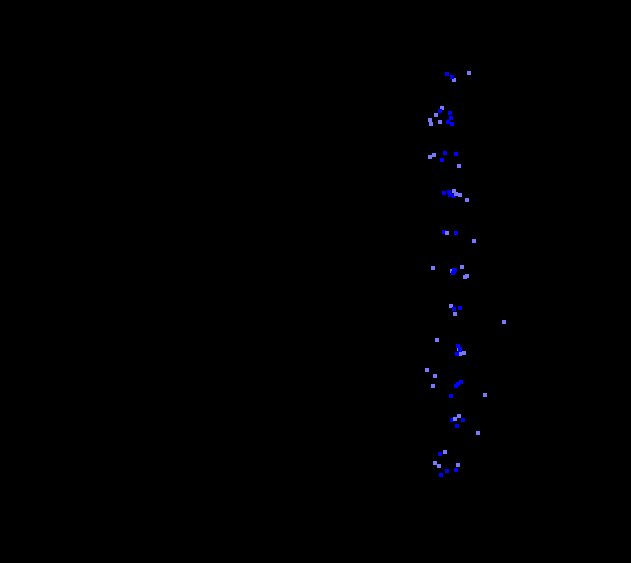
\includegraphics[width=6.8cm]{img/manip_2_4_a.png}
\end{subfigure}%
\begin{subfigure}{7cm}
  \centering
  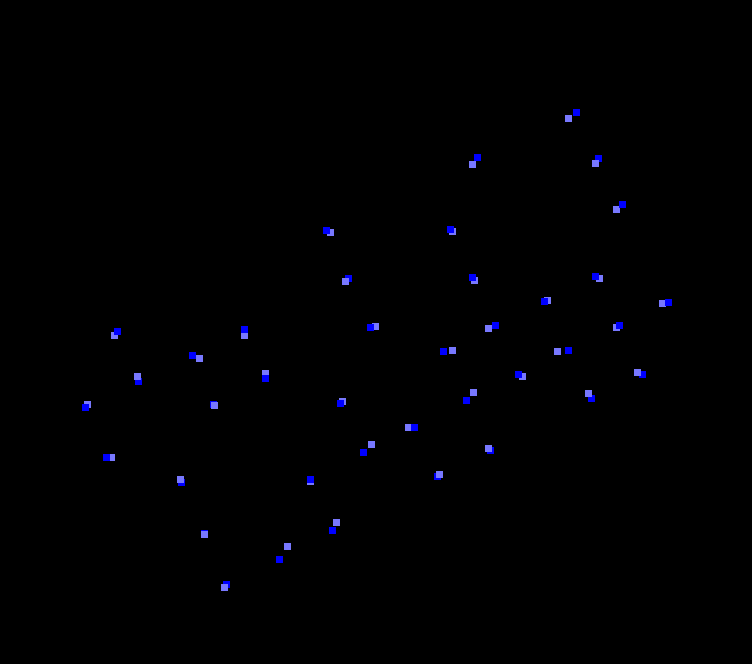
\includegraphics[width=6.8cm]{img/manip_2_4_b.png}
\end{subfigure}
\caption{Left: the ORF reconstructed checkerboard (light blue) is noisier than the stereo one (dark blue) in the $Z$ direction. Right: this effect is less pronounced in the $XY$ plane. The holes are due to rejection of the points considered as too noisy}
\label{fig:manip_2_4}
\end{center}
\end{figure}
A way to check the reliability of the 3D reconstruction is to compute the euclidean distances between each points and compare them to the theoretical $25mm$ of the real checkerboard. In the whole, those distances are always situated around $30mm$ and are bigger for the \gls{ORF} which makes sense because the noise contribution on a distance is always positive and this noise is supposed to be higher with the \gls{ORF}.

In the next part of the process, the sum of the distances between the range finder and the stereo device is minimized and extrinsic matrices are computed. Here, we display the $M_{TL}$ matrices of a calibration using 7 checkerboard capture with the sensors plugged on the Halo.\\
With RANSAC:
\begin{equation}
\begin{pmatrix}[0.7]
0.998 & 0.0465 & 0.0294 & -0.166\\
-0.0456 & 0.999 & -0.0299 & 0.00767\\
-0.0308 & 0.0285 & 0.999 & -0.0589\\
0 & 0 & 0 & 1
\end{pmatrix}
\end{equation}
Without RANSAC:
\begin{equation}
\begin{pmatrix}[0.7]
0.991 & 0.128 & -0.0435 & -0.14\\
-0.128 & 0.992 & -0.00107 & -0.00672\\
0.043 & 0.00663 & 0.999 & -0.0846\\
0 & 0 & 0 & 1
\end{pmatrix}
\end{equation}
In those matrices, we can see that the sensors are pretty aligned (rotation coefficient almost equal to 1 on the diagonal and 0 elsewhere) and we can compare the translations with the theoretical one measured on the CAD model of the \gls{INSPECT} project:
\begin{table}[H]
\begin{center}
\footnotesize
\begin{tabular}{|l|c|c|c|c|}
\hline
 & \multicolumn{2}{c|}{\textbf{CAD Model}} & \multicolumn{2}{c|}{\textbf{Calibration Results}}\\
 \hline
 & in \textit{inches} & in $cm$ & with RANSAC (in $cm$) & without RANSAC (in $cm$)\\
\hline
$X$ & 6.3345 & \textbf{16.09} & \textbf{16.6} & 14\\
\hline
$Y$ & 0.7903 & \textbf{2.01} & \textbf{0.77} & -0.67\\
\hline
$Z$ & 1.8662 & \textbf{4.74} & \textbf{5.89} & 8.46\\
\hline
\end{tabular}
\end{center}
\caption{Comparison of the theoretical and calibration results of the translation between the ORF and the left camera}\label{table:calib}
\end{table}
Given the quality of the sensors and the global mechanical accuracy of the setup, we can consider those results to be quite good. However, it may be important to discuss the limitations:
\begin{itemize*}
\item \textbf{Stereo calibration parameters dependency}: First, as we just reminded, the stereo precision is a function of the focal length $f$ and the baseline $b$ between left and right cameras. Yet, those values are extracted from the stereo calibration and small imprecision on those can increase strongly the error on the final Halo calibration. Indeed, during the triangulation, errors on $b$ and $f$ will cause the reconstructed points cloud to inflate or deflate (figure \ref{fig:manip_2_5}). As the minimization process of this calibration calculate the rotation and translation between the geometric center of each cloud in a way, the calibration will be then dependent on the localization of observed checkerboards (directly influencing the position of the clouds geometric centers). Checkerboard situated essentially along the $X$ axis would lead to a higher error on $X$. In our example, we observe mainly checkerboard along $Z$ but one of them is shifted on the $Y$ axis, which explain the higher error on $Y$. It is important to understand that this problem is only due to the stereo imprecision though. Because of this effect, the global observation drawn among all the calibration tests shows a bigger error on $Z$. As a matter of fact, if the checkerboards photographed during the calibration process are near the center of the $XY$ plane, they have necessarily a positive $Z$ coordinate.
\item \textbf{ORF noise}: Secondly, the noise of the \gls{ORF} is directed along the depth axis and is a function of the luminosity and the materials in the environment. Once again, as the cameras look at checkerboard with a positive $Z$, this component is more concerned by the calibration errors. However, the random nature of this process leads to an error with a zero mean value and then have a lower influence than the previous effect.
\end{itemize*}
% Figure manip_2_5
\begin{figure}[!htt]
\begin{center}
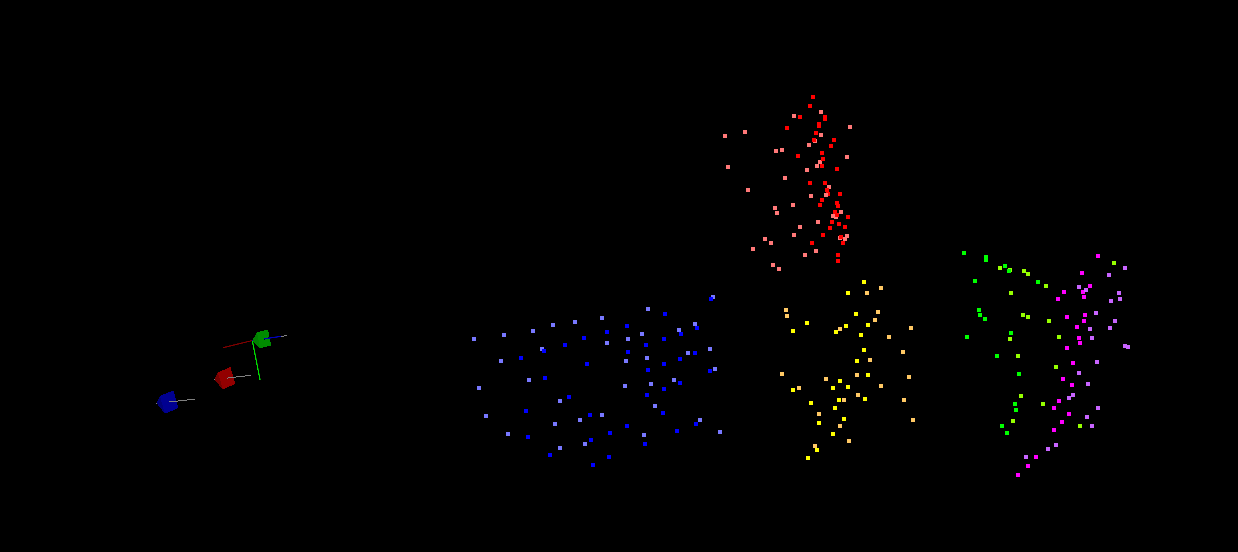
\includegraphics[width=14cm]{img/manip_2_5.png}
\caption{The ORF and stereo reconstructed checkerboard are now superposed thanks to the computed transformation matrix. If we look closely, the ORF checkerboard near the camera is shifted toward the camera when the farthest ORF checkerboard is shifted in the other direction. This highlight the fact that the stereo points cloud is too small, due to stereo calibration parameters inaccuracies}
\label{fig:manip_2_5}
\end{center}
\end{figure}


\section{Sensors Fusion}
\subsection{Ground Results}

1) On montre l'image ORF

2) On montre la division en normales (ici subsampling de 4 pour y voir clair)

3) On montre le resultat final


\subsection{Parabolic Flight Results}

RGA flight: what we can do

\subsection{Discussion}
On peut voir que ca n'apporte rien. Pour 2 raisons:

1) Mouvement

2) extreme non linearity of the projection/triangulation in stereo due to feature matching..

3) Meme dans les cas rare ou ca foncitonne, bcp de parametres a faire varier ainsi que la precision de la calibration: pas reussi a faire en sorte que la probabilite de matching stereo apporte un poids suffisant pour ameliorer la precision de l'ORF, sauf quand lors des false positive que nous voulons justement eviter.


\section{Future Work}

\subsection{Improving Calibration}
-> Improving triangulation
-> Integrate Thermocam:
 - Intrinsic: same method, but checkerboard with the same pattern in IR and visible light ref
 - Extrinsic: Instead of stereo extrinsic calibration, incorporate the thermocam (assuming a ) and calibrate the same way as previously with the couple VERTIGO-thermocam ref

\subsection{Improving this Fusion Algorithm}
-> find better correlation with confidence and sigma
-> ameliorate probability calculus in stereo
-> Integrate Thermocam

\subsection{Building a New Fusion Algorithm}
The real problem of this fusion algorithm: it requires at least good images from the ORF, which seems not to be always true/

-> Keep stereo and ORF in one single process: Invert stereo then orf and interpolation? But this time, we have the opposite problem: when an environment is not textured enough, it won't result
-> Spatial division: parallel reconstruction from ORF and Stereo. then selection of the patchlets? ref and photo
More appropriate 
-> Time division: time => not fusion anymore
